% !TEX encoding = UTF-8 Unicode
\documentclass[11.2pt,twoside]{book}\usepackage[T1]{fontenc}
\usepackage{tikz}

\usepackage[active,tightpage,xetex]{preview}

\usepackage{fontspec,xunicode}

\PreviewEnvironment{pgfpicture}

\setlength\PreviewBorder{0pt}

\usetikzlibrary{calc}

\usetikzlibrary{positioning}



\usepackage{fontspec,xunicode}

\setmainfont{Open Sans Condensed Light}

\def \regionSiete {0.01}
\def \regionCuatro {0.01}
\def \regionTres {0.02}
\def \regionDos {-0.01}
\def \regionOcho {0.00}
\def \regionSeis {0.04}
\def \regionUno{0.13}
\def \regionCinco {0.01}

\definecolor{color1}{RGB}{0,0,128}
\definecolor{color2}{RGB}{100,100,220}
\begin{document}
\begin{tikzpicture}


\node[anchor=south west,inner sep=0] (image) at (0,0) {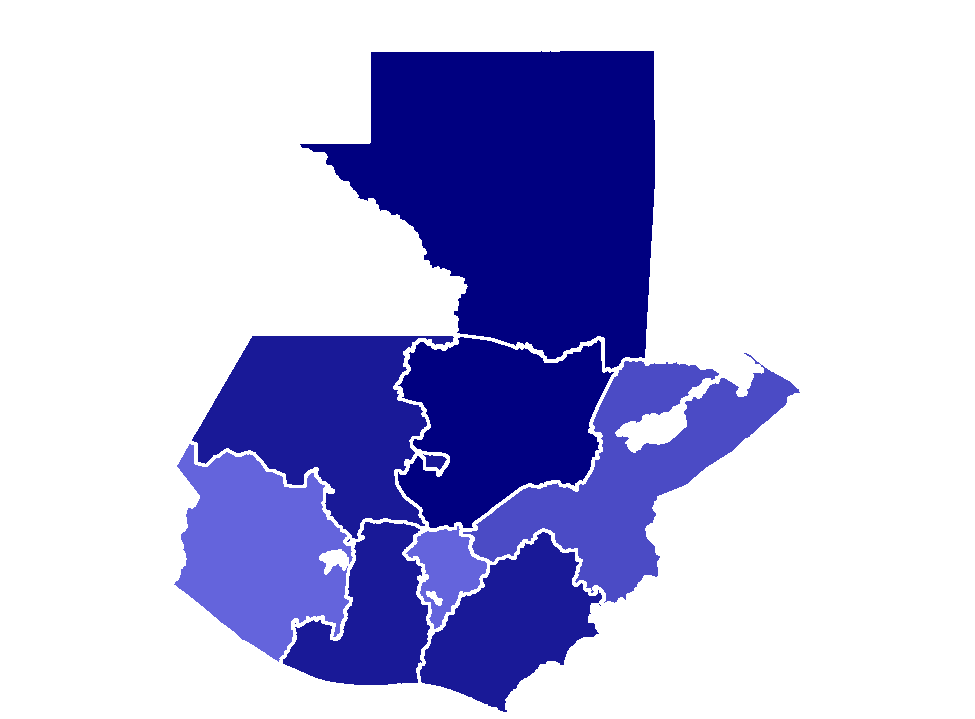
\includegraphics{mapaRegional}};
\begin{scope}[x={(image.south east)},y={(image.north west)}]
%\draw[help lines,xstep=.1,ystep=.1] (0,0) grid (1,1);
%\foreach \x in {0,1,...,9} { \node [anchor=north] at (\x/10,0) {0.\x}; }
%\foreach \y in {0,1,...,9} { \node [anchor=east] at (0,\y/10) {0.\y}; }


%\filldraw[fill=blue!40!white, draw=black] (0,0) rectangle (1,1);








%#############REGION VIII################################# %
\filldraw [gray] (0.55,0.76) circle (1.2pt);
\draw [ gray] (0.55,0.76) -- (0.73,0.76);
\node[text width=3cm, color=gray] at (0.835,0.76) {Región VIII \\  \regionOcho \%};


%#############REGION II################################# %
\filldraw [gray] (0.52,0.41) circle (1.2pt);
\draw [ gray] (0.52,0.59) -- (0.73,0.59);
\draw [gray] (0.52,0.41) -- (0.52, 0.59);
\node[text width=3cm, color=gray] at (0.835,0.59) {Región II \\  \regionDos \%};


%#############REGION III################################# %
\filldraw [gray] (0.64,0.32) circle (1.2pt);
\draw [ gray] (0.64,0.32) -- (0.73,0.32);
\node[text width=3cm, color=gray] at (0.835,0.32) {Región III \\  \regionTres \%};



%#############REGION IV################################# %
\filldraw [gray] (0.52,0.14) circle (1.2pt);
\draw [ gray] (0.52,0.14) -- (0.73,0.14);
\node[text width=3cm, color=gray] at (0.835,0.14) {Región IV \\  \regionCuatro \%};






% ###############REGION VII############################## %
\draw [ gray] (0.34,0.4) -- (0.34,0.83);
\filldraw [gray] (0.34,0.4) circle (1.2pt);
\draw [ gray] (0.34,0.83) -- (0.15,0.83);
\node[align=right,text width=3cm, color=gray] at (0.05,0.83) {Región VII \\ \regionSiete \%};

% ###############REGION VI############################## %
\draw [ gray] (0.28,0.24) -- (0.28,0.69);
\filldraw [gray] (0.28,0.24) circle (1.2pt);
\draw [ gray] (0.28,0.69) -- (0.15,0.69	);
\node[align=right,text width=3cm, color=gray] at (0.05,0.69) {Región VI \\ \regionSeis \%};









% ###############REGION I############################## %
\draw [ gray] (0.46,0.22) -- (0.46,0.1);
\filldraw [gray] (0.46,0.22) circle (1.2pt);
\draw [ gray] (0.46,0.1) -- (0.15,0.1	);
\node[align=right,text width=3cm, color=gray] at (0.05,0.10) {Región I \\ \regionUno \%};

% ###############REGION V############################## %
\draw [ gray] (0.22,0.17) -- (0.22,0.24);
\filldraw [gray] (0.39,0.17) circle (1.2pt);
\draw [ gray] (0.39,0.17) -- (0.22,0.17	);
\draw [ gray] (0.22,0.24) -- (0.15,0.24	);
\node[align=right,text width=3cm, color=gray] at (0.05,0.24) {Región V \\ \regionCinco \%};


\end{scope}


\begin{scope}
\shadedraw[left color=blue,right color=red] (3,3) rectangle (2,2);
\end{scope}

\end{tikzpicture}
\end{document}
